\documentclass[a4paper,14pt]{article}
\usepackage{amssymb}
\usepackage{amsmath}
\usepackage{amsthm}
\usepackage{caption}
\usepackage{enumitem}
\usepackage{misccorr}
\usepackage[noadjust]{cite}
\usepackage{cmap}
\usepackage[utf8x]{inputenc}
\usepackage[T2A]{fontenc}
\usepackage[english, russian]{babel}
\usepackage{graphics}
\usepackage{graphicx}
\usepackage{textcomp}
\usepackage{verbatim}
\usepackage{makeidx}
\usepackage{geometry}
\usepackage{float}
\usepackage{bm}
\usepackage{esint}
\usepackage{mathtools}
\usepackage{graphicx}
\usepackage{listings}
\usepackage{courier}
\usepackage{multirow}
\usepackage{graphicx}
\usepackage{xcolor}
\usepackage{ucs}
\usepackage{titlesec}

\DeclareCaptionLabelSeparator{custom}{ - }

\lstdefinestyle{asm}{
	language={[x86masm]Assembler},
	backgroundcolor=\color{white},
	basicstyle=\footnotesize\ttfamily,
	keywordstyle=\color{blue},
	stringstyle=\color{red},
	commentstyle=\color{gray},
	numbers=left,
	numberstyle=\tiny,
	stepnumber=1,
	numbersep=5pt,
	frame=single,
	tabsize=4,
	captionpos=b,
	breaklines=true
}

\captionsetup[lstlisting]{labelsep=custom}

\lstset{basicstyle=\fontsize{10}{10}\selectfont,breaklines=true,inputencoding=utf8x,extendedchars=\true}

\lstset{
	literate=
	{а}{{\selectfont\char224}}1
	{б}{{\selectfont\char225}}1
	{в}{{\selectfont\char226}}1
	{г}{{\selectfont\char227}}1
	{д}{{\selectfont\char228}}1
	{е}{{\selectfont\char229}}1
	{ё}{{\"e}}1
	{ж}{{\selectfont\char230}}1
	{з}{{\selectfont\char231}}1
	{и}{{\selectfont\char232}}1
	{й}{{\selectfont\char233}}1
	{к}{{\selectfont\char234}}1
	{л}{{\selectfont\char235}}1
	{м}{{\selectfont\char236}}1
	{н}{{\selectfont\char237}}1
	{о}{{\selectfont\char238}}1
	{п}{{\selectfont\char239}}1
	{р}{{\selectfont\char240}}1
	{с}{{\selectfont\char241}}1
	{т}{{\selectfont\char242}}1
	{у}{{\selectfont\char243}}1
	{ф}{{\selectfont\char244}}1
	{х}{{\selectfont\char245}}1
	{ц}{{\selectfont\char246}}1
	{ч}{{\selectfont\char247}}1
	{ш}{{\selectfont\char248}}1
	{щ}{{\selectfont\char249}}1
	{ъ}{{\selectfont\char250}}1
	{ы}{{\selectfont\char251}}1
	{ь}{{\selectfont\char252}}1
	{э}{{\selectfont\char253}}1
	{ю}{{\selectfont\char254}}1
	{я}{{\selectfont\char255}}1
	{А}{{\selectfont\char192}}1
	{Б}{{\selectfont\char193}}1
	{В}{{\selectfont\char194}}1
	{Г}{{\selectfont\char195}}1
	{Д}{{\selectfont\char196}}1
	{Е}{{\selectfont\char197}}1
	{Ё}{{\"E}}1
	{Ж}{{\selectfont\char198}}1
	{З}{{\selectfont\char199}}1
	{И}{{\selectfont\char200}}1
	{Й}{{\selectfont\char201}}1
	{К}{{\selectfont\char202}}1
	{Л}{{\selectfont\char203}}1
	{М}{{\selectfont\char204}}1
	{Н}{{\selectfont\char205}}1
	{О}{{\selectfont\char206}}1
	{П}{{\selectfont\char207}}1
	{Р}{{\selectfont\char208}}1
	{С}{{\selectfont\char209}}1
	{Т}{{\selectfont\char210}}1
	{У}{{\selectfont\char211}}1
	{Ф}{{\selectfont\char212}}1
	{Х}{{\selectfont\char213}}1
	{Ц}{{\selectfont\char214}}1
	{Ч}{{\selectfont\char215}}1
	{Ш}{{\selectfont\char216}}1
	{Щ}{{\selectfont\char217}}1
	{Ъ}{{\selectfont\char218}}1
	{Ы}{{\selectfont\char219}}1
	{Ь}{{\selectfont\char220}}1
	{Э}{{\selectfont\char221}}1
	{Ю}{{\selectfont\char222}}1
	{Я}{{\selectfont\char223}}1
}

%opening
\title{}
\author{Цховребова Яна Роландовна}

% геометрия
\geometry{pdftex, left = 3cm, right = 10mm, top = 2cm, bottom = 2cm}

\setcounter{tocdepth}{4} % фикс переноса 
\righthyphenmin = 2
\tolerance = 2048

\begin{document}
	
\begin{titlepage}
	\noindent
	\begin{tabular}{|c|c|}	
	\hline
	\noindent	
	\begin{minipage}{0.14\textwidth}
		
\includegraphics[width=\linewidth]{assets/logo}
	\end{minipage} &
	\noindent
	\begin{minipage}{0.75\textwidth}\centering
		\textbf{\newline Министерство науки и высшего образования Российской Федерации}\\
		\textbf{Федеральное государственное бюджетное образовательное учреждение высшего образования}\\
		\textbf{«Московский государственный технический университет имени Н.Э.~Баумана}\\
		\textbf{(национальный исследовательский университет)»}\\
		\textbf{(МГТУ им. Н.Э.~Баумана)}
	\end{minipage} \\
	\hline	
	\end{tabular}
	\newline\newline\newline\newline\newline\newline
	\noindent ФАКУЛЬТЕТ~~~ \underline{~~~~~~~~~~~~~~~~~~~~~~~~~~~~~«Информатика и системы управления»~~~~~~~~~~~~~~~~~~~~~~~~~~~~~} \newline\newline
	\noindent КАФЕДРА~~~~~~~ \underline{~~~~~~~~~~«Программное обеспечение ЭВМ и информационные технологии»~~~~~~~~~~~~} \newline\newline
	\noindent НАПРАВЛЕНИЕ ПОДГОТОВКИ~~~ \underline{~~~~~~~~~~~~~~~~~«09.03.04 Программная инженерия»~~~~~~~~~~~~~~~~~~} \newline\newline
	
	\vspace{2.5cm}
	
	\begin{center}
		\Large\textbf{\textsc{ОТЧЕТ}}\\
		\Large\textbf{\textsc{по лабораторной работе №1}}\\
	\end{center}
	
	\vspace{1cm}
	
	\noindent\textnormal{НАЗВАНИЕ} \hspace{10mm} \underline{\textnormal{~~~~~~~~~~~~~~~~~~~~~~~~~~~~~~~~~~~~~~~~~~Прерывание INT 8h~~~~~~~~~~~~~~~~~~~~~~~~~~~~~~~~~~~~~~~}}\noindent

	\vspace{1.3cm}
	
	\noindent\textnormal{ДИСЦИПЛИНА} \hspace{3mm} \underline{\textnormal{~~~~~~~~~~~~~~~~~~~~~~~~~~~~~~~~~~~~~~~~~Операционные системы~~~~~~~~~~~~~~~~~~~~~~~~~~~~~~~~~~~~}}\noindent
	
	\vspace{2cm}
	
	\noindent\textnormal{Студент} \hspace{25mm}
	\underline{\textnormal{{~~~ИУ7-54Б~~~}}}
	\hspace{17mm}
	\underline{\textnormal{\hphantom{~~~~~~~~~~~~~~~~~~~~~~~~~~~~~~~~}}} \hspace{6mm}
	\underline{\textnormal{~~~~Цховребова Я.Р.~~~~}}
	
	\vspace{2mm}
	
	\noindent\textnormal{\hphantom{Студент}} \hspace{30mm}\noindent
	\fontsize{8pt}{8pt}
	\textnormal{Группа}\hspace{35mm}\textnormal{Подпись, дата} \hspace{22mm}\noindent\textnormal{Фамилия И. О.}
	
	\vspace{0.5cm}
	
	\fontsize{12pt}{12pt}\selectfont
	\noindent\textnormal{Преподаватель} \hspace{50mm}
	\underline{\textnormal{\hphantom{~~~~~~~~~~~~~~~~~~~~~~~~~~~}}} \hspace{5mm}
	\noindent\underline{\textnormal{~~~Рязанова Н.Ю.~~~}}
	
	\vspace{2mm}
	
	\noindent\textnormal{\hphantom{Студент}} \hspace{28mm}\noindent
	\fontsize{8pt}{8pt}
	\textnormal{}\hspace{45mm}\textnormal{Подпись, дата} \hspace{22mm}\noindent\textnormal{Фамилия И. О.}
	
	\vspace{0.5cm}
	
	\fontsize{12pt}{12pt}\selectfont

	\begin{center}
		\vfill
		Москва, ~\the\year
		~г.
	\end{center}
	\clearpage
\end{titlepage}

\section{Дизассемблированный код}
\subsection{Обработчик прерывания INT 8h} 

\begin{lstlisting}[style={asm}, caption={Листинг прерывания INT 8h}]
	020C:0746  E8 0070				call	sub_2			; (07B9)
	020C:0746  E8 70 00				db	0E8h, 70h, 00h
	020C:0749  06					push	es
	020C:074A  1E					push	ds
	020C:074B  50					push	ax
	020C:074C  52					push	dx
	020C:074D  B8 0040				mov	ax,40h
	020C:0750  8E D8				mov	ds,ax
	020C:0752  33 C0				xor	ax,ax			; Zero register
	020C:0754  8E C0				mov	es,ax
	020C:0756  FF 06 006C				inc	word ptr ds:[6Ch]	; (0040:006C=0F4D7h)
	020C:075A  75 04				jnz	loc_1			; Jump if not zero
	020C:075C  FF 06 006E				inc	word ptr ds:[6Eh]	; (0040:006E=2)
	020C:0760			loc_1:
	020C:0760  83 3E 006E 18			cmp	word ptr ds:[6Eh],18h	; (0040:006E=2)
	020C:0765  75 15				jne	loc_2			; Jump if not equal
	020C:0767  81 3E 006C 00B0			cmp	word ptr ds:[6Ch],0B0h	; (0040:006C=0F4D7h)
	020C:076D  75 0D				jne	loc_2			; Jump if not equal
	020C:076F  A3 006E				mov	word ptr ds:[6Eh],ax	; (0040:006E=2)
	020C:0772  A3 006C				mov	word ptr ds:[6Ch],ax	; (0040:006C=0F4D7h)
	020C:0775  C6 06 0070 01			mov	byte ptr ds:[70h],1	; (0040:0070=0)
	020C:077A  0C 08				or	al,8
	020C:077C			loc_2:
	020C:077C  50					push	ax
	020C:077D  FE 0E 0040				dec	byte ptr ds:[40h]	; (0040:0040=3Dh)
	020C:0781  75 0B				jnz	loc_3			; Jump if not zero
	020C:0783  80 26 003F F0			and	byte ptr ds:[3Fh],0F0h	; (0040:003F=0)
	020C:0788  B0 0C				mov	al,0Ch
	020C:078A  BA 03F2				mov	dx,3F2h
	020C:078D  EE					out	dx,al			; port 3F2h, dsk0 contrl output
	020C:078E			loc_3:
	020C:078E  58					pop	ax
	020C:078F  F7 06 0314 0004			test	word ptr ds:[314h],4	; (0040:0314=3200h)
	020C:0795  75 0C				jnz	loc_4			; Jump if not zero
	020C:0797  9F					lahf				; Load ah from flags
	020C:0798  86 E0				xchg	ah,al
	020C:079A  50					push	ax
	020C:079B  26: FF 1E 0070			call	dword ptr es:[70h]	; (0000:0070=6ADh)
	020C:07A0  EB 03				jmp	short loc_5		; (07A5)
	020C:07A2  90					nop
	020C:07A3			loc_4:
	020C:07A3  CD 1C				int	1Ch			; Timer break (call each 18.2ms)
	020C:07A5			loc_5:
	020C:07A5  E8 0011				call	sub_2			; (07B9)
	020C:07A8  B0 20				mov	al,20h			; ' '
	020C:07AA  E6 20				out	20h,al			; port 20h, 8259-1 int command
	;  al = 20h, end of interrupt
	020C:07AC  5A					pop	dx
	020C:07AD  58					pop	ax
	020C:07AE  1F					pop	ds
	020C:07AF  07					pop	es
	020C:07B0  E9 FE99				jmp	$-164h
	;; <...>
	020C:064C			loc_5:
	020C:064C  1E					push	ds
	020C:064D  50					push	ax
	;; <...>
	020C:06AA  58					pop	ax
	020C:06AB  1F					pop	ds
	;; <...>
	020C:06AC  CF					iret				; Interrupt return
\end{lstlisting}
\clearpage
\subsection{Процедура sub\_2}
\begin{lstlisting}[style={asm}, caption={Листинг процедуры sub\_2}]
	020C:07B9			sub_2		proc	near
	020C:07B9  1E					push	ds
	020C:07BA  50					push	ax
	020C:07BB  B8 0040				mov	ax,40h
	020C:07BE  8E D8				mov	ds,ax
	020C:07C0  9F					lahf				; Load ah from flags
	020C:07C1  F7 06 0314 2400			test	word ptr ds:[314h],2400h	; (0040:0314=3200h)
	020C:07C7  75 0C				jnz	loc_7			; Jump if not zero
	020C:07C9  F0> 81 26 0314 FDFF	                           lock	and	word ptr ds:[314h],0FDFFh	; (0040:0314=3200h)
	020C:07D0			loc_6:
	020C:07D0  9E					sahf				; Store ah into flags
	020C:07D1  58					pop	ax
	020C:07D2  1F					pop	ds
	020C:07D3  EB 03				jmp	short loc_8		; (07D8)
	020C:07D5			loc_7:
	020C:07D5  FA					cli				; Disable interrupts
	020C:07D6  EB F8				jmp	short loc_6		; (07D0)
	020C:07D8			loc_8:
	020C:07D8  C3					retn
	sub_2		endp
\end{lstlisting}
\section{Схемы алгоритмов}
\subsection{Схема алгоритма обработчика INT 8h}

\begin{flushright}
	\begin{center}
		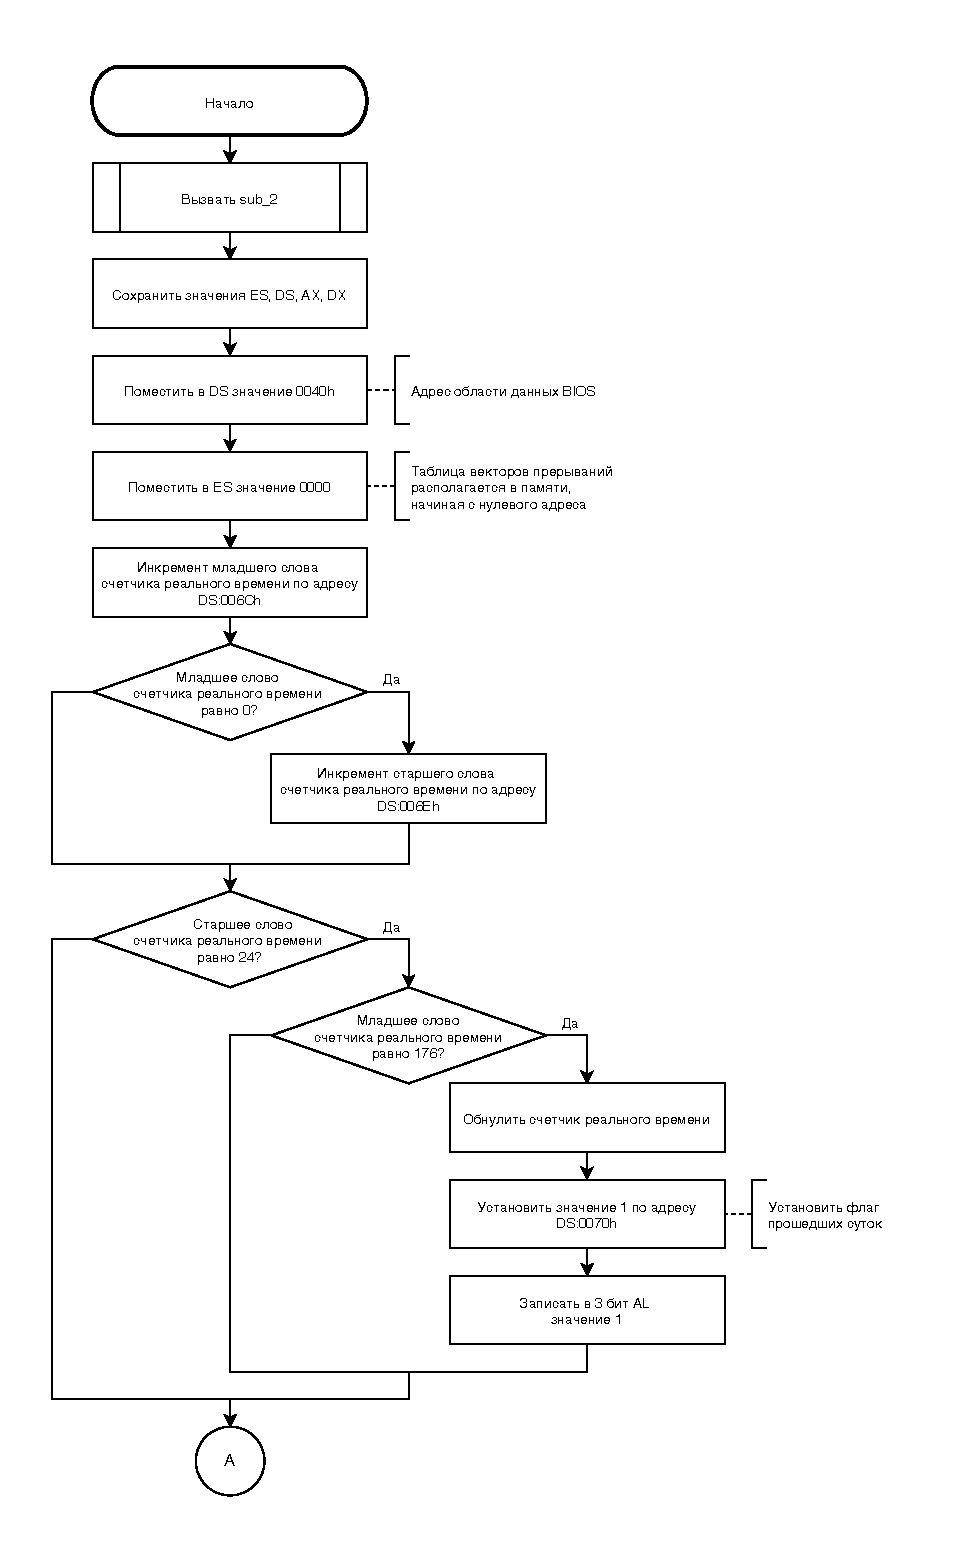
\includegraphics[height=0.98\textheight]{assets/int8h_part1.pdf}
	\end{center}
	\begin{center}
	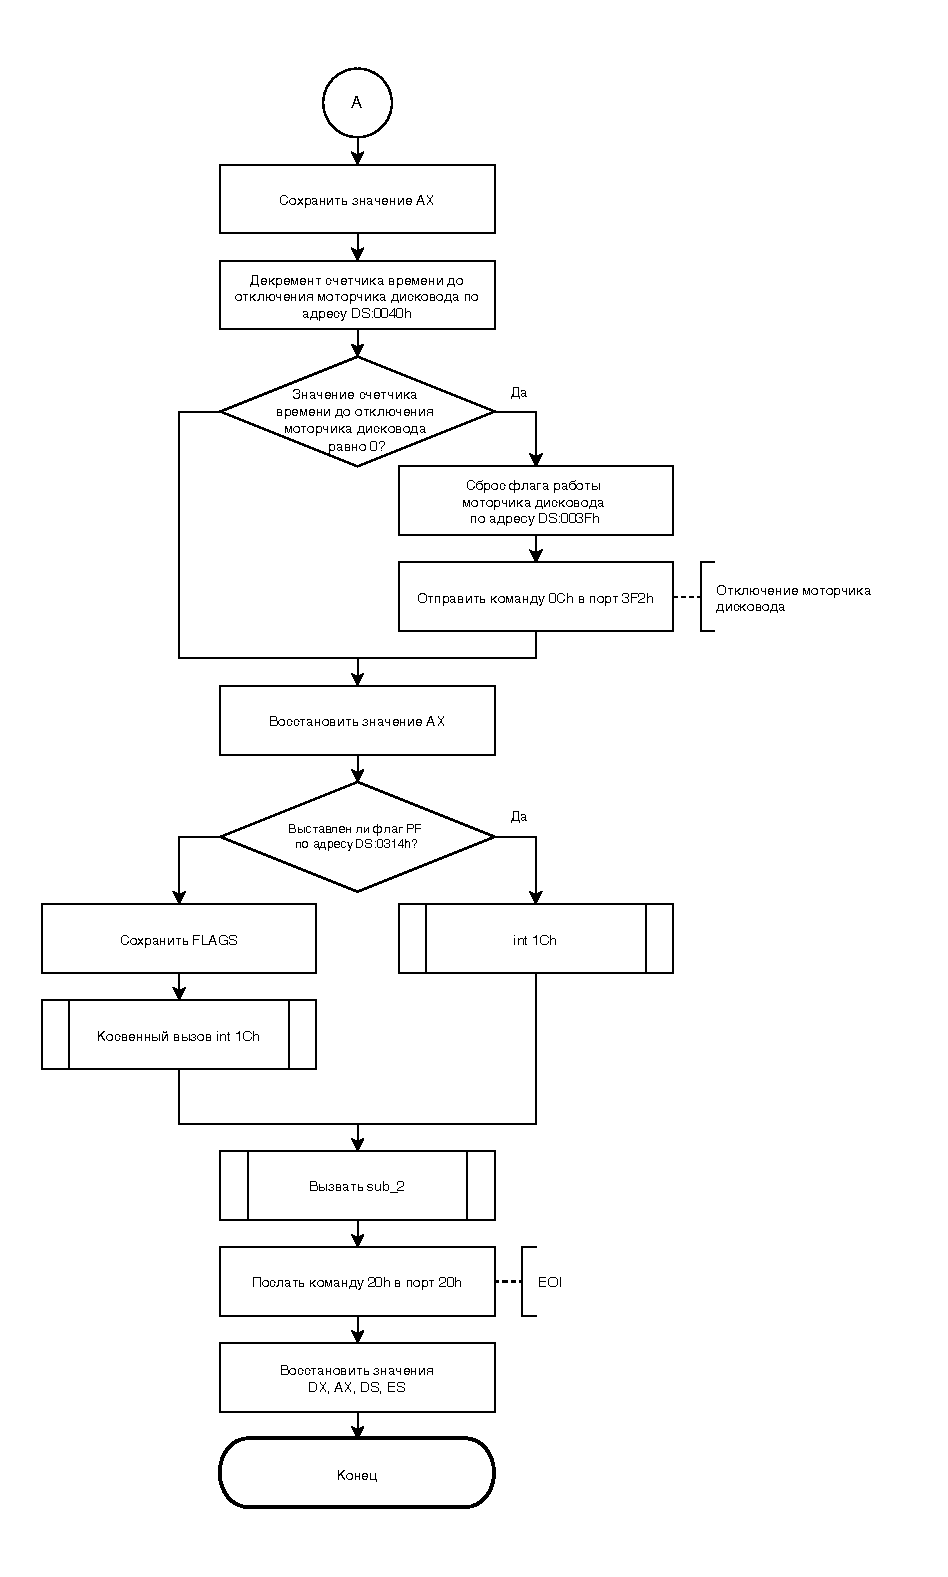
\includegraphics[height=0.98\textheight]{assets/int8h_part2.pdf}
	\end{center}
\end{flushright}

\newpage

\subsection{Схема алгоритма процедуры sub\_2}

\begin{flushright}
	\begin{center}
		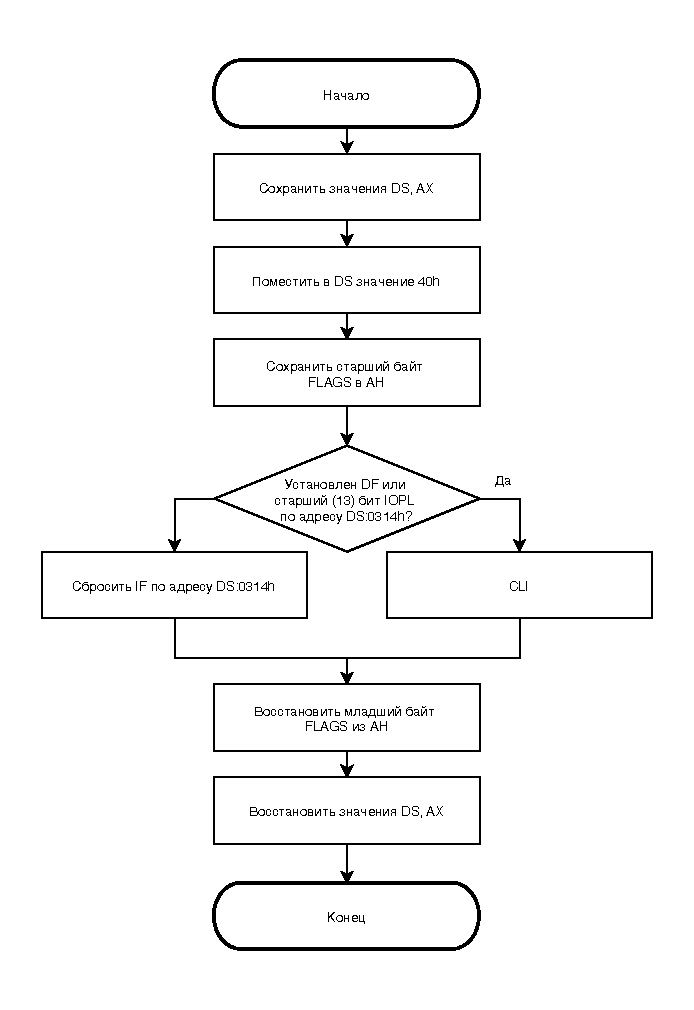
\includegraphics[height=0.8\textheight]{assets/sub_2.pdf}
	\end{center}
	\clearpage
\end{flushright}
	
\end{document}
